Area AM inactivation
The inactivation results are consistent with hemispatial neglect. This makes sense if my hypothesis is correct that visual area AM is the same area as the stereotactic position of mouse PPC. (I now have some preliminary widefield imaging data to support this hypothesis). A couple of lesion studies in rats show that unilateral lesion of PPC (left or right) causes spatial neglect.  I haven’t looked into whether this also generalizes to mice.

Hemispatial neglect would argue against the idea that inactivation causes the animals to perceive more flashes, rather the inactivation results would suggest that the mice are neglecting the tendency to go towards the affected visual hemifield, which corresponds to the same location where they would respond to for higher flashes. To test this idea, training animals on the reverse contingency should yield the same effect, i.e. a bias ipsilateral to the stimulation hemisphere which would correspond to low number of flashes.

Another set of experiments to test this idea further is to train mice on a task with two interspersed conditions: instructed and free choice. In the instructed trials the animal are given an LED cue at the reward port (left or right) and in the free choice trials, both LEDs are turned on and the animal can go to any port to receive the reward. According to literature on PPC lesions/inactivations in humans, primates, and rats, PPC inactivation should only affect (i.e. bias the subject) on free choice trials and not the instructed trials. Since this should be an easy task for the animals to acquire, I could use this same task but perturb another visual area, for example V1 and the expected outcome would be the opposite effect, i.e. bias on instructed trials and no effect on free choice.
%-----------------------------------------------------------------------------

\subsection{d' (d-prime)}
Another quantitative measure of psychophysical performance is \emph{d'} (pronounced d prime), also known as the discriminability or sensitivity index. \emph{d'} is a dimensionless statistic that quantifies the separation between the means of a signal and noise distribution \parencite{Macmillian,Green1989SignalPsychophysics} (Equation \ref{dprime1}). 

%-----------------------------------------------------------------------------
For a logistic distribution,
\begin{equation}
	\centering
	F(x;\alpha,\beta) = \frac{1}{1 + \exp(-(\alpha + \beta x))}
\end{equation}
$\alpha$ and $\beta$ are the regression coefficients that represent the bias and slope and of the psychometric function, respectively. For logistic distribution, the bias can be mapped into units of the stimulus (Equation \ref{bias}), and is equivalent to the point of subjective equality (PSE) or threshold.  
\begin{equation}
	\centering
	PSE =  -\frac{\alpha}{\beta}
    \label{bias}
\end{equation}
%-----------------------------------------------------------------------------
%hesitant to include psychophysical kernels,
\begin{figure}
  \centering
  	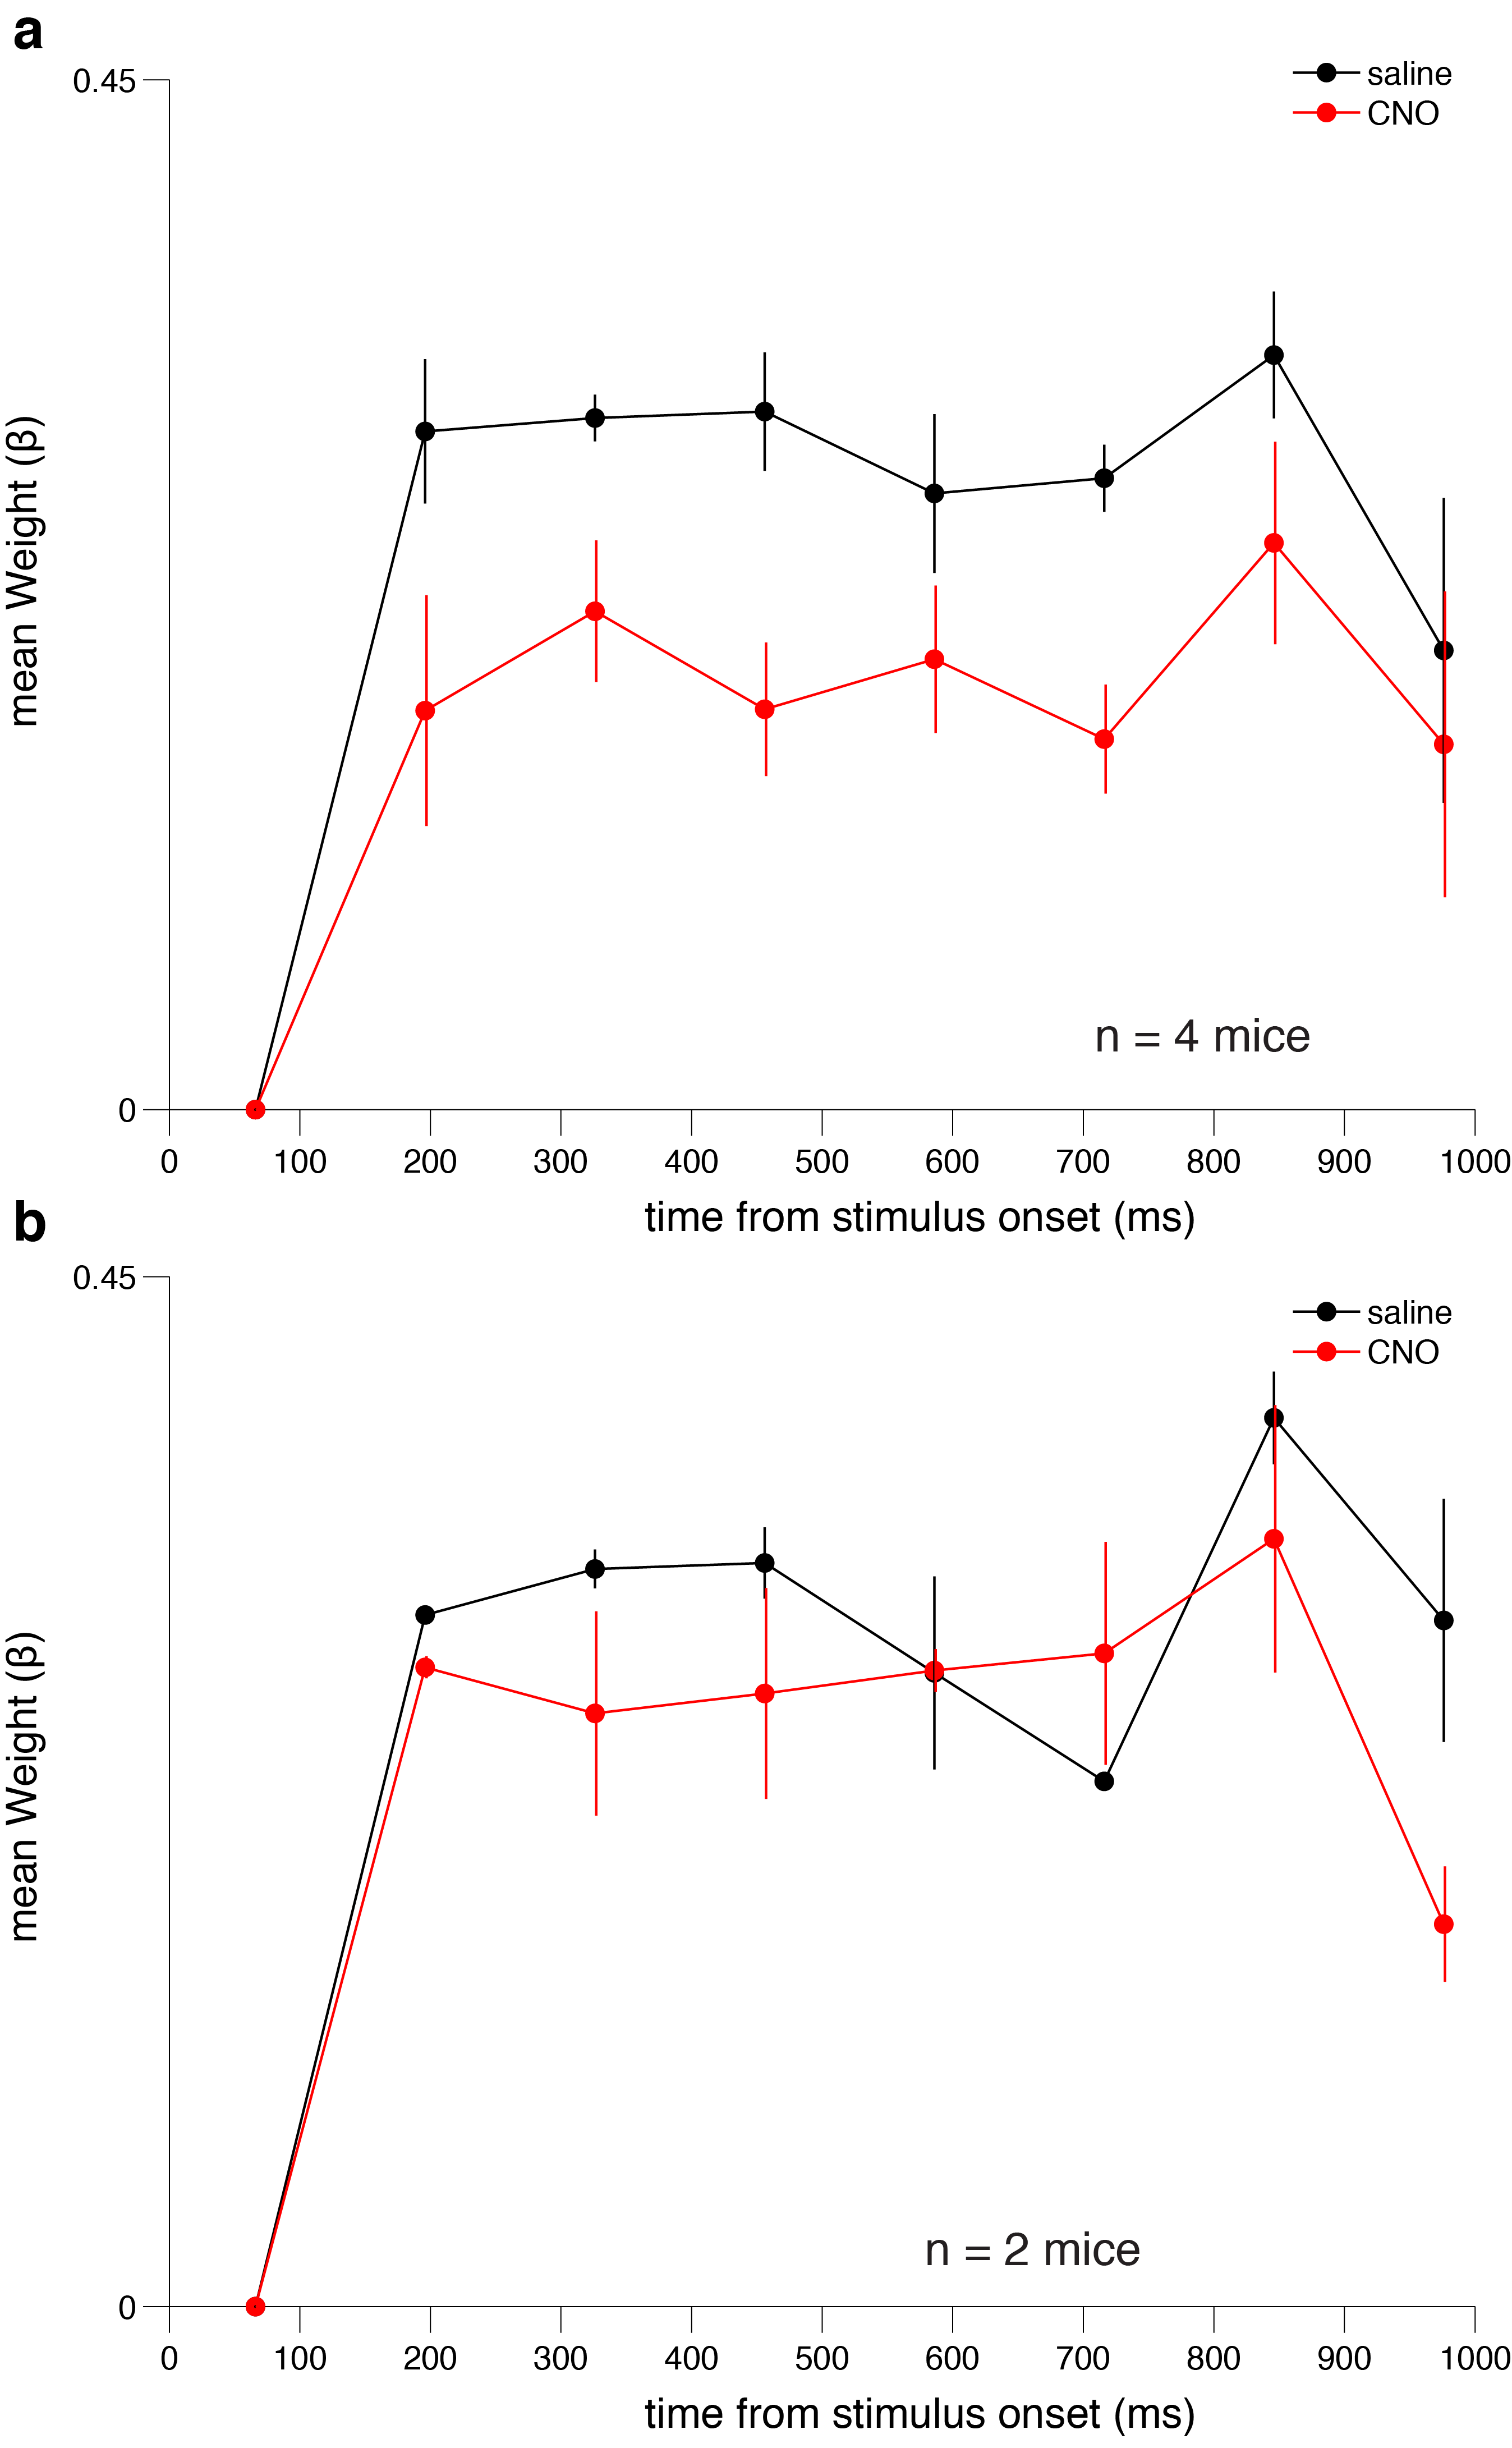
\includegraphics[scale=0.3]{Figures/chapter3/psychophysical_kernel_sem_dreaddandcontrol.png}
  \caption[Reverse Correlation Psychophysical Kernel]{Psychophysical kernel estimated by reverse correlation, indicating the relative contribution of flashes occurring at different time points on the subject's choice. (a) Average kernel for DREADD-expressing group and (b) control group.}
   \label{fig:dreaddkernel}
\end{figure}
Another approach to evaluate DREADD manipulation effects over time is by estimating the psychophysical kernel. The psychophysical kernel reflects the relative influence of stimulus flashes presented at different times on the subject's choice. For example, if the flashes presented earlier in the trial are more informative, the psychophysical weightings would be greater earlier than later in trial. We used a logistic regression approach described in Chapter \ref{Chapter2} \parencite{Katz2016DissociatedStream} to perform the reverse correlation analysis and estimate the psychophysical kernel.  On average, the temporal profiles of the psychophysical kernels were similar on CNO vs. saline sessions, however, DREADD PPC disruption reduced psychophysical weightings over time (Figure \ref{fig:dreaddkernel}a), which was not observed in the control group (Figure \ref{fig:dreaddkernel}b).

The near uniform reduction in the psychophysical weightings (kernel) observed on CNO sessions compared to saline sessions (Figure \ref{fig:dreaddkernel}a) is reminiscent of the weightings reduction found when area MT was inactivated during a visual evidence accumulation task in nonhuman primates \textcite{Katz2016DissociatedStream}. Area MT is a visual area involved in motion processing and perception \parencite{Albright1984DirectionMacaque,Newsome1988AOf}. Similarly, mouse (rodent) PPC could also be playing a sensory role ie. processing of visual information, rather than integration or accumulation of evidence \parencite{Licata2016PosteriorRats}.